\chapterauthor{Scott Klasky, Jackie Chen, et al}{ORNL, Sandia}

\chapter{S3D/ADIOS Case Study}
\label{part4-ch5-s3d}

Please target 5-6 pages for this chapter (including figures+references). Readers should be able to appreciate why the application is interesting and lessons learnt from the case study.

\section{Science Use Case}
Describe the science/end-user goal. What is challenging about the application? Describe the data model.
Are there any unique aspects about this application? 

\section{Software and Hardware}
What platforms did you use? What software did you use? Was there any specific reason to choose specific I/O middleware or library?

\section{Performance}
You can provide details about your experimental setup. What I/O performance did you obtain? 

\index{Parallel I/O}
\index{Combustion}
\index{AMR}

\begin{figure}[h!]
\centering
\myIfColor
{
% use color version
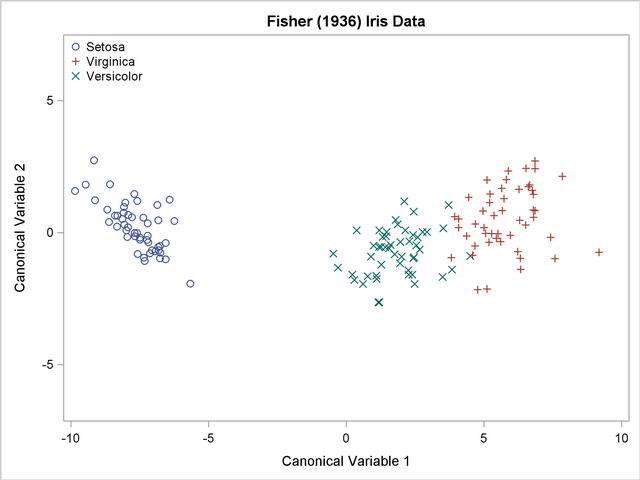
\includegraphics[width=0.99\textwidth]{Chapters/part4-ch5-s3d/figs/canonical.png}
}
{
% use B&W version
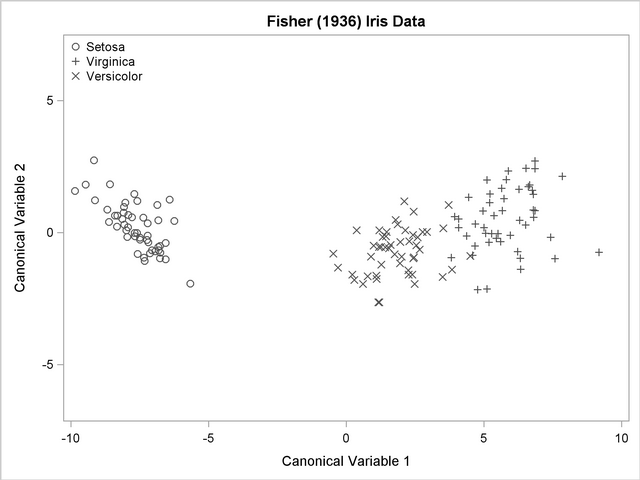
\includegraphics[width=0.99\textwidth]{Chapters/part4-ch5-s3d/figs/canonical-bw.png}
}
\caption[Placeholder caption for compelling image.]
{Placeholder caption for compelling image. \ImageCourtesyOf{John Doe (AAA)}.
}
\label{part4-ch5-s3d:fig:image1}
\end{figure}

\section{Conclusion}
Are you happy with the I/O performance. Any lessons learnt from the exercise? Would you have done things differently next time around? 

%This is a reference to a book chapter~\ref{ch0:book-intro}.
This is a reference to a bibtex item~\cite{Snir:MPI}.

\putbib[Chapters/part4-ch5-s3d/part4-ch5-s3d]
